\newcommand{\pwd}{key}

\renewcommand{\password}{key\xspace}

We introduce the problem  through an example, and outline our
approach.  We work with a  small, class-based object-oriented language similar to Joe-E \cite{JoeE} with modules,   module-private fields
({accessible} only from   methods {from} the same module)
initalised by a class's implicit constructor,
with unforgeable and un-enumerable addresses.
%Classes have an 
%with appropriate default values.
%KJX YEAH COS we were going to use inappropriate values?
%
We distinguish between  \emph{\internalO}
objects --- instances of our internal module $M$'s classes ---
and \emph{\externalO} objects defined in
\emph{any} number of external modules $\overline M$. 
{\prg{Private} methods  {may only be} called by objects of the same
  module,  while \prg{public}  methods  may be called by \emph{any}
  object with a reference to the method receiver, {and with
  actual arguments of  dynamic types that match} the declared formal parameter types.} 
% SD dropped
% Our model of execution is entirely unsurprising with a stack, a heap, and states.
\footnote{As in Joe-E, we leverage  module-based privacy to restrict propagation of capabilities, and reduce the need for reference monitors etc, \cf Sect 3 in  \cite{JoeE}.}   

% \subsubsection{Internal and external modules, objects, and states}
 \label{s:concepts}

We are concerned with guarantees made in an \emph{open} setting; that
is, our internal module
$M$ must be programmed so that 
its execution, together with any external modules $\overline M$
will uphold these guarantees.
$M$ must ensure these guarantees hold
whenever the
$\overline M$  \emph{\externalM} modules are executing,
yet without relying on any assumptions about $\overline M$'s code
(beyond the programming language's semantics)%
\footnote{
This is a critical distinction from e.g.\
co{\"o}perative approaches such as rely/guarantee
\cite{relyGuarantee-HayesJones-setss2017,relyGuarantee-vanStaden-mpc2015}.}.
The internal module may break these guarantees temporarily,
so long as they \sdN{are re{\"e}stablished} before (re)entry to an external module.
 

% \kjx{haven't mentioned states yet, so this is too early --- We also distinguish between
%      \emph{\internalC} and   \emph{\externalC} states - those whose receiver is internal or external respectively. }
 
 

\subsection{\prg{Shop} -- illustrating tamed effects} % Reason about external calls (using protection)}
\label{sec:how}
\label{sec:shop}

The challenge when calling a method on an external object, is that we have no specification for that method. 
 For illustration, consider the following, internal, module \Mshop, and assume that it includes the classes \prg{Item}, \prg{Shop}, \prg{Account}, and \prg{Inventory}. 
Classes  \sdN{\prg{Inventory} and \prg{Item} have the expected functionality. 
\prg{Account}s hold a balance and have a \password. 
With access to an \prg{Account}, %'s address, 
one  can pay money into it, 
and with access to an account  and its \password, one can withdraw money from that account.
Implementations of such a class  appear in the next section.
}
 \prg{Shop}  has  a public method \prg{buy} whose formal parameter \prg{buyer} is an \prg{external}   object. 
 % SD chopped  with a method { \prg{pay}.}} 

\begin{lstlisting}[mathescape=true, language=Chainmail, frame=lines]
module M$_{shop}$
  ...   
  class Shop
    field accnt:Account, invntry:Inventory, clients:[external]    
  
    public method buy(buyer:external, anItem:Item)
      int price = anItem.price
      int oldBlnce = this.accnt.blnce
      buyer.pay(this.accnt, price)     // $\red{\mbox{external\ call}}!$
      if (this.accnt.blnce == oldBlnce+price)  this.send(buyer,anItem)
      else
         buyer.tell("you have not paid me") 
     
      private method send(buyer:external, anItem:Item)  
       ... 
        
\end{lstlisting}
 

The critical point is the external call on line 9,   \sdN{where the \prg{Shop} asks the \prg{buyer} to pay the price of that item,
by calling  \prg{pay} on \prg{buyer} and passing its account as an argument.
As \prg{buyer} is an external object, the module \Mshop has no method specification for \prg{pay}, and no 
certainty about what its implementation %knowledge of what the implementation of \prg{pay} 
might do. 
}

\sdN{What are the possible effects of that external call?}
% How can we reason about this external call?
\sdN{The \prg{Shop} hopes, but cannot be sure, that at line 10  it  will have received money; but 
it wants to be certain  that   the \prg{buyer} will not use this opportunity and the access to the 
shop's account  to drain its moneys.
Can \prg{Shop}  be certain?}

\vspace{.1cm}
% \noindent
Indeed, if \Mshop  makes appropriate guarantees, it can \tame  the effects at line 9. In particular,  
 \\
$\strut \ \ \ (A)\ \ $ If \Mshop guarantees that no money can be withdrawn from an account unless the external\\  
$\strut \ \ \ \ \ \ \ \ \ \ \ $ object causing the withdrawal can eventually get access to the account's \password, \ \ \  \se{\emph{and}} \\
$\strut \ \ \ (B)\ \ $  if \prg{buyer} cannot eventually get access to the account's \password,   \ \ \    \se{\emph{ then}}  \\
$\strut \ \ \ (C)\ \ $ The external  call on line 9 will not cause a reduction in the shop's account's balance.


\vspace{.3cm}
\sdN{The remit of our work is to provide the formal specification and verification tools to support arguments as the one given above. 
\footnote{\sdN{TODO: elaborate here on ``can eventually get acces'', and on ``tamed effect''}}
In the argument above, we used the, not yet defined, concept of  "can  eventually get access to", and assumed \tamed effects (no money withdrawn ... unless ..). 
We need need to define these concepts, and develop Hoare Logics for reasoning.
Therefore, we need to address the following four challenges:}
\begin{description}
\item[\ \ \ \ \  1$^{st}$ Challenge] The specification   of ``can eventually get access to''. 

\item[\ \ \ \ \   2$^{nd}$ Challenge] The specification of tamed effects, 

\item[\ \ \ \ \  3$^{rd}$ Challenge] A  Hoare Logic for external calls,

\item [\ \ \ \ \   4$^{th}$ Challenge]  A Hoare Logic for proving that modules adhere to specifications
\end{description}

\vspace{.2cm}
\noindent
 \textbf{NOTE} \sdN{One might think that  wrapping the account so as to allow payments but forbid withdrawals, would be sufficient  to \tame the possible effects on line 9. 
However, such a wrapper might not be sufficient, as the
% nece\tame the effects because
 \prg{buyer} might  have access to the account and its \password even before the call to \prg{pay}. 
}

 
 
\subsection{1$^{st}$ Challenge: eventual access} 

\sdN{We propose  the concept of \emph{protection} to  describe  lack of access. We say that $o$ is \emph{protected}, if external objects  cannot obtain direct access to $o$ unless some internal object affords that access.}

 \begin{description}
\item[Protection] Object $o$ is \emph{protected} from $o'$, formally $\protectedFrom {o} {o'}$,  
 if the penultimate object on any path from $o$ to $o'$  is internal.
% if $o'$ cannot obtain direct access to $o$ unless an internal object affords that access. %to $o$. 
Object $o$ is \emph{protected}, formally ${\inside{\prg{\it{o}}}}$, if $o$ is protected from all external objects transitively accessible from the currently executing method call. %More in 
-- \cf Defs. \ref{def:chainmail-protection-from}, \ % and 
\ref{def:chainmail-protection}.
 \end{description}
 
 \sdN{Program execution may turn protected objects to un-protected, but this may only be caused by execution of an internal method -- hence only internal objects can afford that access.}

Figure \ref{fig:ProtectedBoth} illustrates  protection. \sdN{The left pane shows a heap with objects $o_1$-$o_9$; green resp. pink objects are internal resp. external;  arrows indicate fields.} 
Here  $o_1$, $o_4$, $o_5$ and $o_9$ 
are protected from $o_2$. 
 The middle pane \sdN{shows the same heap and a stack with frame  $\phi_1$} whose receiver,   \prg{this},  points to $o_1$. Here 
 $o_1$, $o_2$, $o_4$, $o_5$ and $o_9$  are protected. 
 The right pane \sdN{shows the same configuration, but after pushing frame  $\phi_2$}, whose receiver,  \prg{this},  and local variable, \prg{x}, point to $o_3$ and  $o_7$ resp.
 Here $o_3$ and $o_7$ are protected.  in addition  to  the objects protected in the previous pane. 



\begin{figure}[htb]
\begin{tabular}{|c|c|c|}
\hline
\resizebox{4.5cm}{!}{
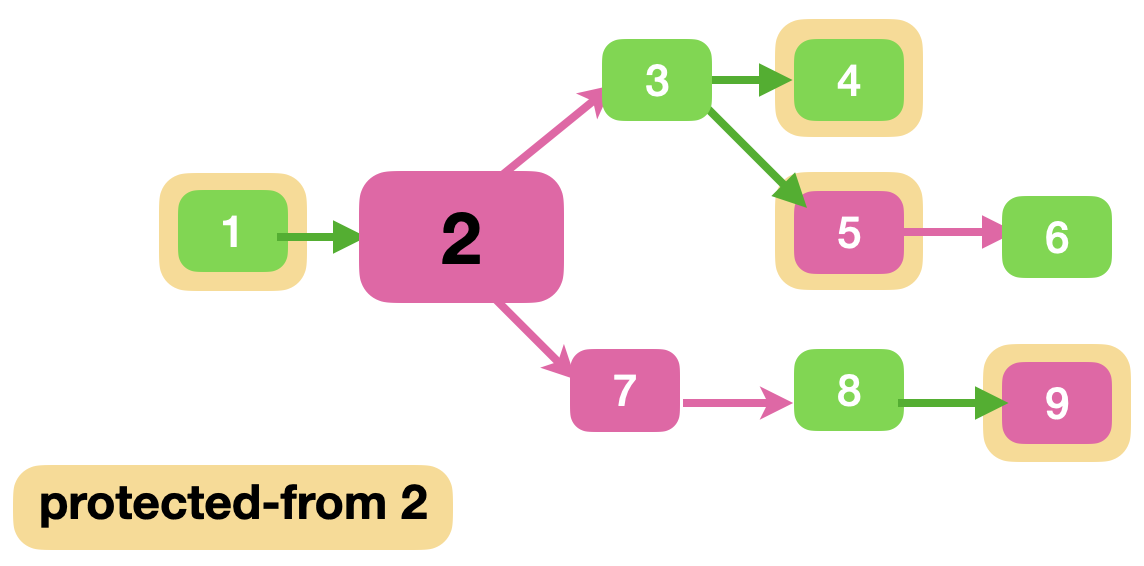
\includegraphics[width=\linewidth]{diagrams/prfC.png}
} 
&
\resizebox{4.5cm}{!}{
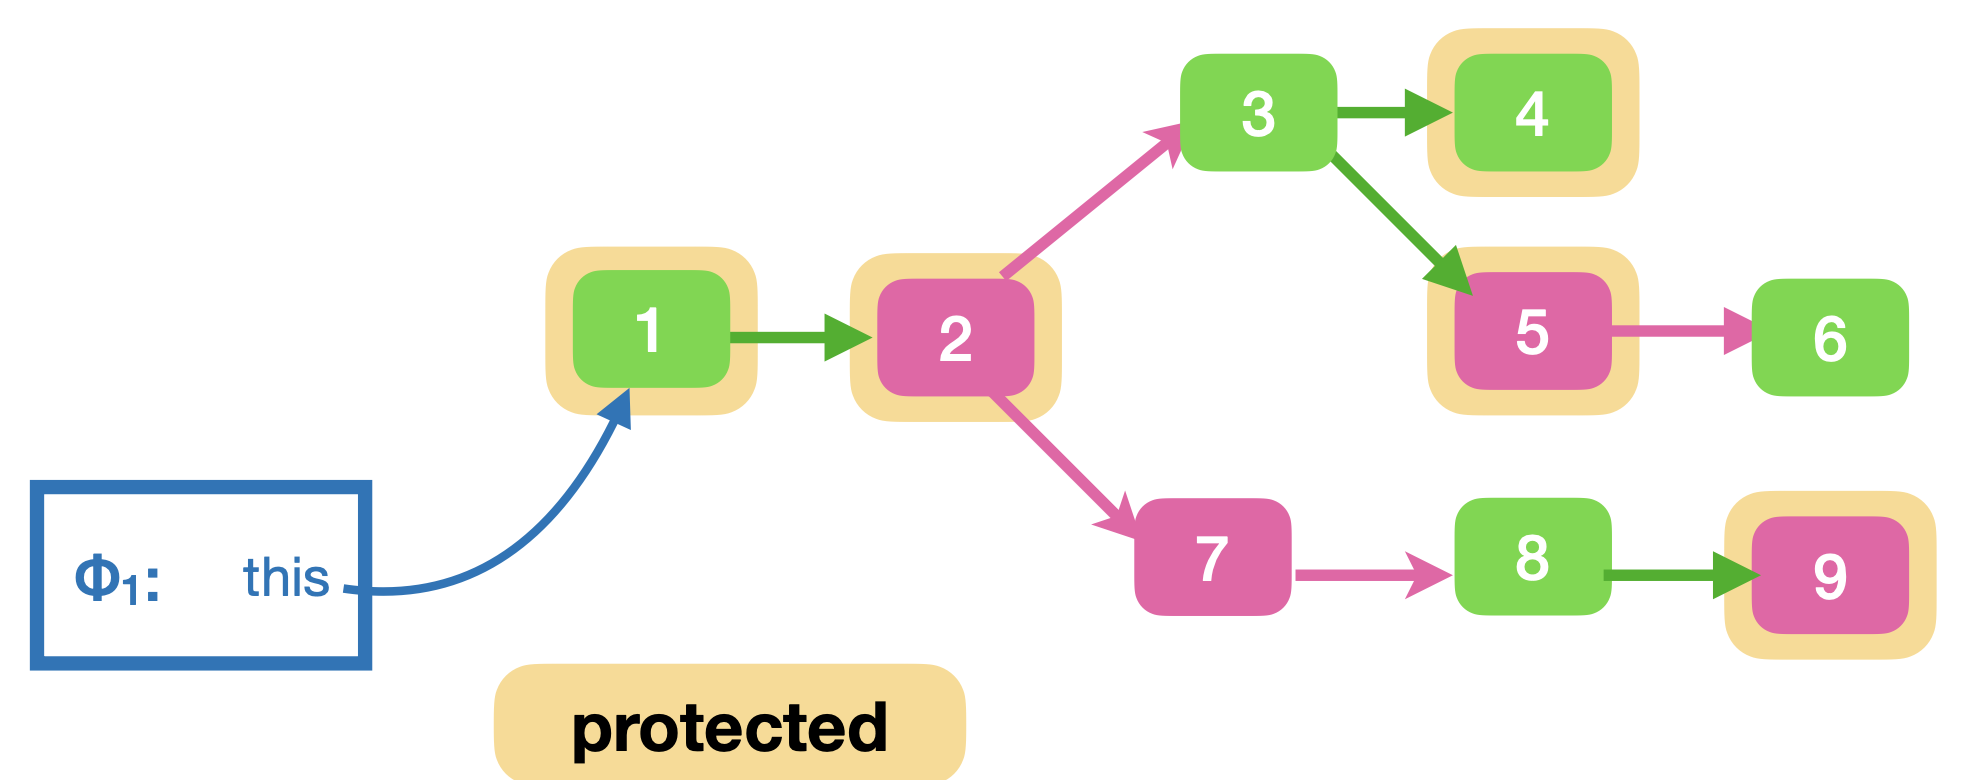
\includegraphics[width=\linewidth]{diagrams/prtFirst.png}
}
&
\resizebox{4.5cm}{!}{
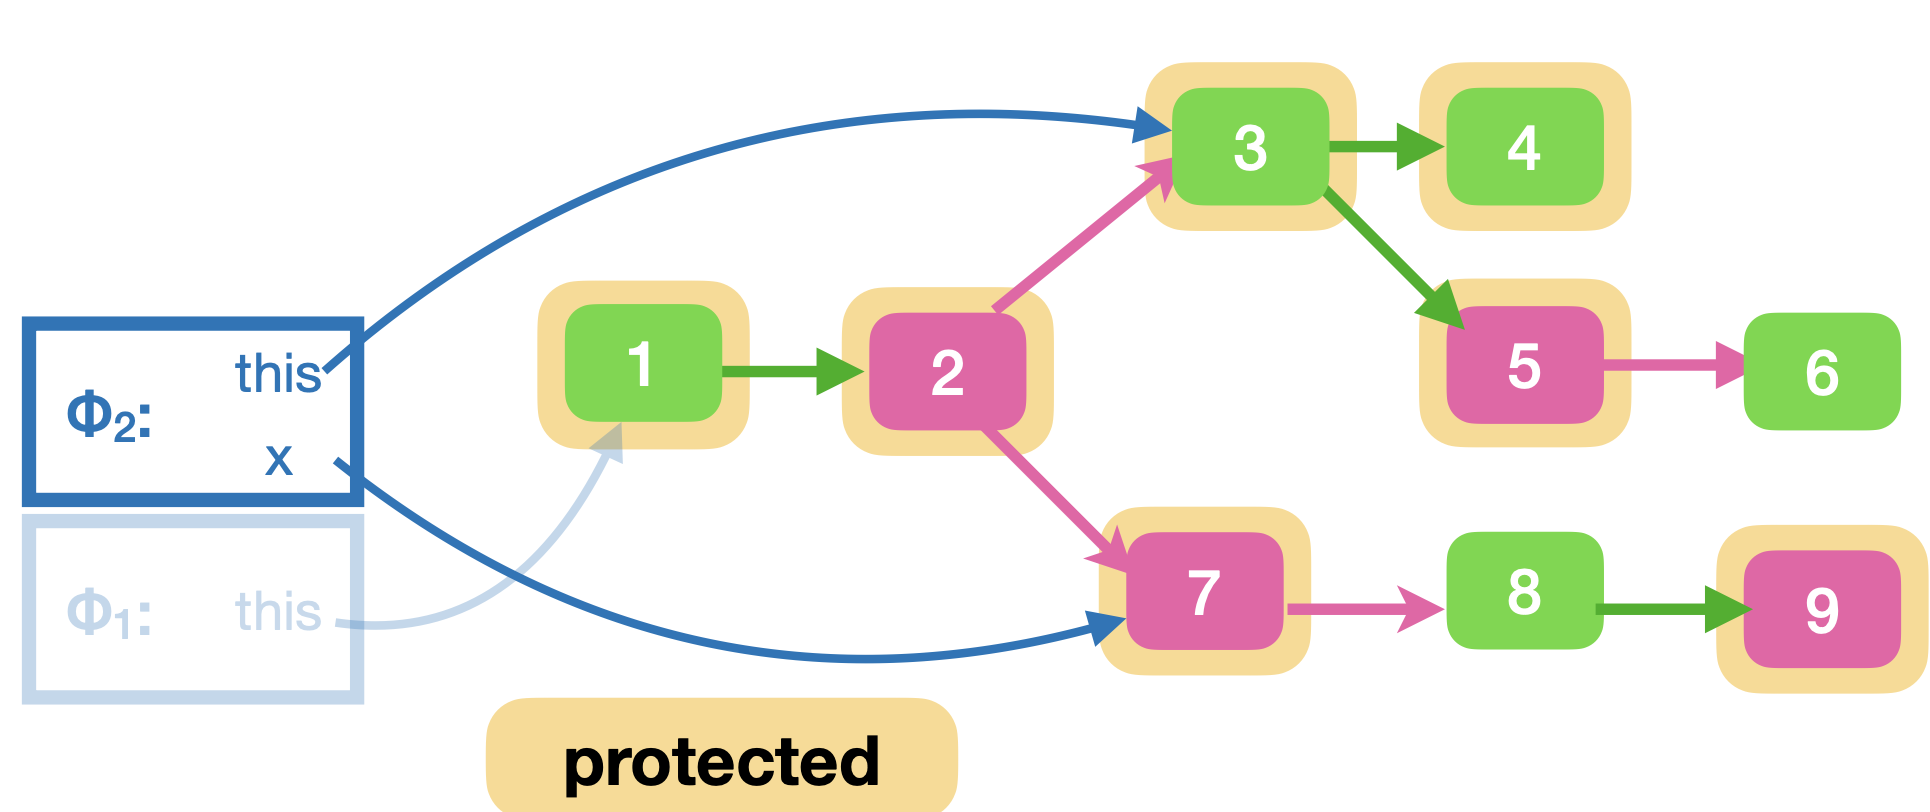
\includegraphics[width=\linewidth]{diagrams/prtSecond.png}
}
\\
\hline
protected from object $o_2$
&
protected  with top frame $\phi_1$
&
protected  with top frame $\phi_2$
\\
\hline \hline
\end{tabular}
   \caption{Protected from, and Protected. Pink resp. green squares are external resp. internal objects. Connecting straight arrows  indicate fields. Blue boxes are frames on the stack. Protected objects   highlighted in yellow.}
   \label{fig:ProtectedBoth}
 \end{figure}
 

\subsection{2$^{nd}$ Challenge: Specification of tamed effects}

How can we express the guarantee that effects are \tamed? %some effects will not happen? 
 In particular, when such effects can be the outcome of the execution of more than one method? Traditional PRE/POST condition specifications cannot express guarantees that two or more of our methods won't interact to produce an untamed effect. 
%
We build on the concept of two-state invariants, and define

\begin{description}
\item[{Scoped invariants}] %describe emergent behaviour:  
{$\TwoStatesN  {\overline{x:C}}  {A}$} expresses that if a {state} $\sigma$ 
 has objects $\overline x$ of class $\overline C$, and satisfies $A$, then all $\sigma$'s \emph{scoped  future  states} will  {also} satisfy  {$A$}. 
The scoped future  {contains all states which can be reached through any steps, including further method calls and returns, but stopping before returning} from the call active in $\sigma$ --  \cf Def  \ref{def:shallow:term}.
%{We} consider executions of the internal module linked with any number of unknown, external modules,
%-- \cf Sect. \ref{sect:execution}.
% SD: I dropped sentence above; too much detail, I thought!
\sdN{For} $\sigma$ and its scoped future   we only consider external states -- \cf Def \ref{def:necessity-semantics}.
\end{description}

    
\label{s:bank}
\label{s:bankSpecEx}

\newcommand{\SPSP}{\ \ \ \ \ \  \ \ \ \  }
\noindent
For example, the following scoped invariants\\
$\strut \SPSP  S_1\ \  \triangleq \ \ \TwoStatesN {\prg{a}:\prg{Account}}  {\inside{\prg{a}}} $ 
\\
$\strut  \SPSP  S_2\ \  \triangleq \ \ \TwoStatesN  {\prg{a}:\prg{Account}}  {\inside{\prg{a.key}}} $ 
 \\
$\strut  \SPSP   S_3\ \  \triangleq \ \ \TwoStatesN {\prg{a}:\prg{Account},\prg{b}:\prg{int}}  {\inside{\prg{a}} \wedge \prg{a.\balance}=\prg{b}}  $
\\
$\strut  \SPSP  S_4\ \  \triangleq \ \ \TwoStatesN{ \prg{a}:\prg{Account},\prg{b}:\prg{int} } {\inside{\prg{a.key}} \wedge \prg{a.\balance} \geq \prg{b} } $
 
% \end{tabular}
%}

\noindent
%specifications
 give the  guarantees:\\
 $\strut  \SPSP  S_1$:\   accounts are not leaked, \\
$\strut   \SPSP S_2$:\    keys are not leaked,\\
$\strut \SPSP  S_3$:\  the balance is not modified unless there is unprotected access to the account,  \\%while 
$\strut \SPSP  S_4$:\   the balance does not decrease unless there is unprotected access to the key.  


 
\vspace{.1cm}

\begin{example}
We illustrate the meaning of our specifications  using three  versions of a class \prg{Account}  from  \cite{OOPSLA22} 
as part of our internal module \Mshop. 
To differentiate, we rename \Mshop  as $\ModA$,  $\ModB$, or $\ModC$. 
All use the same \prg{transfer} method for withdrawing money.
%All use the same method \prg{transfer} to  withdraw money, only when supplied with the key.
\forget{All versions {use the same method \prg{transfer} to} allow  withdrawal of money, only when supplied with the key to the account.
All use the same method \prg{transfer} to  withdraw money, only when supplied with the key.}
%Moreover, in $\ModA$ the key is immutable, in $\ModB$ it is unconditionally mutable, while in $\ModC$ the key may be modified, but only if supplied with the old key. 

%\emph{Guarding} is the crucial expectation that comes with object capabilities. \footnoteSD{SAY THIS BETTER?} 
%Hoare logics support the specification of    enabling of effects (through per-method PRE/POST-condition pairs), but not of guarding of effects.
%The latter % specification of capabilities as guards 
%requires per-module guarantees, as proposed, \eg,  in \cite{OOPSLA22}, and in also the current work.
%\footnoteSD{BOLD! Birkedahl and Dreyer might scream!}
%
% \vspace{.1cm}
\begin{lstlisting}[mathescape=true, language=Chainmail, frame=lines]
module $\ModA$      
  class Shop   ... as earlier ...
  class Key
  class Account
    field blnce:int 
    field key:Key
    public method transfer(dest:Account, key':Key, amt:int)
      if (this.key==key')
        this.blnce-=amt
        dest.blnce+=amt
     public method set(key':Key)
      if (this.key==null)  this.key=key'
\end{lstlisting}

Now consider  modules \ModB and \ModC who differ from \ModA only in their \prg{set} methods. Whereas \ModA 's key is immutable, \ModB allows any client to reset an account's key at any time, and \ModC requires the existing key in order to change it.
  

\begin{tabular}{lll}
\begin{minipage}[b]{0.40\textwidth}

\begin{lstlisting}[mathescape=true, language=Chainmail, frame=lines]
$\ModB$
public method set(key':Key)
  this.key=key'
\end{lstlisting}
\end{minipage}
&\ \ \  \ \   &%
\begin{minipage}[b]{0.48\textwidth}
\begin{lstlisting}[mathescape=true, language=chainmail, frame=lines]
$\ModC$
public method set(key',key'':Key)
  if (this.key==key')  this.key=key''
\end{lstlisting}
\end{minipage} 
\end{tabular}

{Thus, in all three modules, the key is an object capability which \emph{enables} the withdrawal of the money. 
Moreover, in $\ModA$ and $\ModC$, the key
\sdN{is a capability} used to  \emph{tame} withdrawal of money, preventing those without it from getting the money from the account.}
Crucially,  in $\ModB$ the key \emph{does not tame} withdrawal of money.
Using $\ModB$, it is possible to start in a state where the account's key is unknown, modify the key, and then withdraw the money. 
% This is not possible  in $\ModA$ and $\ModC$.
% \noindent
%Although the \prg{transfer} method is the same in
%all three modules,   
Code  {such as}
\\ 
$\ \strut \hspace{.2in} $ \prg{k=new Key;  acc.set(k); acc.transfer(rogue\_accnt,k,1000)} 
\\ 
is enough to drain  \prg{acc} in \ModB without knowing the \password.\footnoteSD{CAREFUL: we had 
$\ \strut \hspace{.01in} $ \prg{an\_account.set(42); an\_account.transfer(rogue\_accnt,42)} but this was type incorrect!}
 
 \emph{Emergent behaviour} is key here: 
Even though % the method 
\prg{transfer} in  \ModB is ``safe'' when considered in isolation, it is not safe when considered in conjunction with other methods from the same module. 
Our  specifications  rule  out \ModB while permitting \ModA and
\ModC:
All three modules satisfy $S_1$ and $S_3$. Modules $\ModA$ and $\ModC$ also satisfy $S_2$ and $S_4$, while $\ModB$ satisfies neither $S_2$ nor $S_4$.
\end{example}
 
 \noindent
% \textbf{NOTE} \ \  
 Our specifications are  in terms of the complete module, rather than per-method.
 They talk about externally observable effects (\eg the key stays protected), 
 % the account's balance may increase), 
 rather than about  individual methods (\eg\, \prg{set}). %  or \prg{transfer}).
{Thus,  % gives our specifications the the vital advantage that our specifications can % be used to constrain
  they can characterize  any 
module with  accounts which have a % {\textit{implementation}} of a bank account with a 
 \balance~and a \password -- even as ghost fields --}  irrespective of the API offered.
 % , services  exported, or  dependencies on other parts of the system.\footnoteSD{does this come from OOPSLA? if so we need to rephrase}
%\notesep
%Adherence to   specifications is not monotonic:
%{Eg, while  \ModA satisfies $S_4$, the addition of \prg{set} lead to \ModB, which does not.}
%% Adding a method to a module does not necessarily preserve such adherence,
%% \eg adding method \prg{set} in module \ModB breaks 
%%SD removed the below. When we changed the invaraints to have the same assertion re and post it no longer hel
%\forget{, and while separate methods may adhere to a  specification, their combination does
%not necessarily do so. 
%{For example, \ModB's  \prg{tansfer} and \prg{set} satisfy $S_4$, but their interplay does not.}
%%In this sense, and, similar to OOPSLA'22, our  specifications capture a module's \emph{emergent behaviour}. 

  
  \subsection{3$^{rd}$ Challenge:  A Hoare logic for external calls} %  (using scoped invariants)}
 \label{sec:howThird}
 
 When reasoning about external calls, even though we do not have a specification for the call, we know that the effects of the call are tamed according to the module's scoped invariants. That is expressed in the  simplified Hoare rule below -- \cf. Fig.\ref{f:external:calls}. 
 
  $\inferruleNoName  
 	{ 
   	   {\TwoStatesN {\overline {x:D}} {A}}\ \   \mbox{is part of $M$'s specification}
        }
	{   \triple { \    { \external{y_0}} \,     \wedge \,  \overline{x:D}\  \wedge\  A\ }  
						{ \ u:=y_0.m(y_1,.. y_n)\    }
						{ \    A  \ }
						\  \  ...
         }
$

\vspace{.1cm}

 We now  revisit the external call from line 9 in Section \ref{sec:shop}. Our argument is that if the module satisfies $S_4$, and if before calling \prg{pay}, the \password\ of the shop's account is protected from \prg{buyer}, then, after the call, the balance of that account will not have decreased. 
 That is, we want to be able to establish   a Hoare triple of the form
 \\
$\strut \ \ \ \ \ \ \ \ \ \ \  \{\  \ { \external{\prg{buyer}}} \ \wedge\ {\protectedFrom {\prg{this.\myAccount.key}} {\prg{buyer}}\ \wedge\ {\prg{this.\myAccount.\balance}}=\prg{b}    }\ \  \}$\\
$\strut \ \ \ \ \ \ \ \ \ \ \   \ \ \ \ \ \ \ \ \ \ \ \ {\ \prg{buyer.pay(this.accnt,price)}   \ } $\\
$\strut \ \ \ \ \ \ \ \ \ \ \  \{\  \ \  {\prg{this.\myAccount.\balance}} \geq  \prg{b} \  \  \}$ 

We cannot directly apply the Hoare rule as given above. Namely, to apply $S_4$, we need to establish  
${\inside {\prg{this.\myAccount.key}}}$, and  $\prg{this.\myAccount.\balance}\geq\prg{b}$. 
The latter can be done through the rule of consequence. 
But what about the former? 
We only know that $\protectedFrom {\prg{this.\myAccount.key}} {\prg{buyer}}$, but   need the stronger property  ${\inside {\prg{this.\myAccount.key}}}$. 

 {While we cannot be certain that \prg{this.\myAccount.key} 
 {is  protected during execution of \prg{buy}\footnote{\sdN{What if one of the \prg{clients} had access to it?}}, we are certain that it  \emph{is} protected during execution} of \prg{pay}: 
This is so, because the   accessible objects in the execution of \prg{pay} are those accessible from \prg{buyer}.
{In general, more objects are protected from the viewpoint of the callee than from the viewpoint of the caller. -- cf Fig.  \ref{fig:ProtectedBoth}.
To express this,} we define the operator $\pushSymbolAA$ , which   translates an assertion from the viewpoint of the callee, to that of the caller:
 $\PushAS y A$   guarantees that $A$ will hold when the values of variables $\overline y$ have been pushed onto a new frame. 
 In particular,   $\PushAS y {(\inside \re)} =  \protectedFrom \re {\overline {y} }$ for any term  $\re$ -- \cf 
 Def. \ref{def:push},  and Lemma \ref{lemma:push:ass:state}.
Here we have that 
 $\PushASLong {\{\prg{buyer},\prg{price}\}}  {(\inside {\prg{this.\myAccount.key}})}$
 =  $\protectedFrom {\prg{this.\myAccount.key}} {(\prg{buyer},\prg{price})}$.}


 {Below we show another   Hoare logic rule %\ruleExtCallB\ from
dealing with external calls -- \cf. Fig.\ref{f:external:calls} }
 
 $\inferruleNoName  
 	{ 
   	   {\TwoStatesN {\overline {x:D}} {A}}\ \   \mbox{is part of $M$'s specification}
        }
	{   \triple { \    { \external{y_0}} \,     \wedge \,  \overline{x:D}\  \wedge\  {\PushAS {y}{A}}\ }  
						{ \ u:=y_0.m(y_1,.. y_n)\    }
						{ \    {\PushAS {y}{A}}  \ }
						\  \  ...
         }
$

 
 
 
   \subsection{4$^{th}$ Challenge: A Hoare Logic for Proving that modules adhere to specifications} %  (using scoped invariants)}

 We now revisit the meaning of scoped invariants: 
  {$\TwoStatesN  {\overline{x:C}}  {A}$} expresses that if an external {state} $\sigma$ 
% with objects $\overline x$ of class $\overline C$ 
 satisfies $\overline {x:A} \wedge A$, then all its \emph{scoped} external future  states will  {also} satisfy  {$A$}. 
\Eg if $\sigma$ was an external state executing a call to \prg{Shop::buy}, then a \emph{scoped} external future  state
 could be an external state reachable 
after the return from \prg{Shop::buy}, but could also be reachable
during execution of the external call \prg{pay}.
This means that we are  interested in the states before %and after a method (or statements)
statements, \emph{but  also}  in the external states reachable \emph{during} execution of these statements. 
%of that method (or statements).
To accommodate this, we extend   traditional Hoare triples to quadruples of  form\\
 $\strut \ \hspace{4cm} \quadruple {A} {\, stmt\, }{A'} {A''}$\\  
 promising that if a state satisfies $A$ and executes $stmt$, any terminating state will satisfy $A'$, and 
 and  any intermediate external states reachable during execution of $stmt$ satisfy    $A''$ -- \cf Def. \ref{def:hoare:sem}.
% same as above, but ugly line break:
% terminating execution of $stmt$ in  states satisfying $A$  reaches    final states satisfying $A'$, and any intermediate external states reachable during execution of $stmt$ satisfy    $A''$ -- \cf Def. \ref{def:hoare:sem}.

\vspace{.05cm}

The Hoare logic rule from earlier dealing with external calls is:
 
 $\inferruleNoName  
 	{ 
   	   {\TwoStatesN {\overline {x:D}} {A}}\ \   \mbox{is part of $M$'s specification}
        }
	{   \quadruple { \    { \external{y_0}} \,     \wedge \,  \overline{x:D}\  \wedge\  {\PushAS {y}{A}}\ }  
						{ \ u:=y_0.m(y_1,.. y_n)\    }
						{ \    {\PushAS {y}{A}}  \ }
						{\  A  \ }
         }
$

\vspace{.1cm}

To develop our logic, we     assume a  Hoare logic of  triples, whose assertions do not known the concept of protection.
We then extend this logic as follows: We define an embedding into our quadruples. 
and allow method specifications which also talk about intermediate external states.
We add substructural rules, rules talking about protection,   rules about internal and external calls, 
and the module's adherence to its 
specification - more in Figs. \ref{f:underly} -  \ref{f:calls}. % \ref{f:wf}.
 
 \vspace{.1cm}
A module is well-formed, if  its invariants are well-formed,    its public methods preserve   its invariants, and  all  methods satisfy their specifications - \cf  Fig.  \ref{f:wf}.
%
An invariant is well-formed if % the constituent assertion 
it is \emph{encapsulated}, \ie can only be invalidated by internal code %from that module 
-- \cf Def. \ref{d:encaps}. 
%For example, in \ModA the assertion  \prg{a.balance}$\geq$\prg{b} is encapsulated, but it would not be encapsulated 
%% in a module \ModD   implements balances through a third party, openly accessible ledger 
%if balances were in an external, openly modifiable ledger -- \cf Ex. \ref{ex:not:encaps}.
% 
A method preserves an assertion   if it preserves it   from pre- to  post-states and also to any intermediate external state.

\vspace{.1cm}
\Eg to prove  that method \prg{Shop::buy} satisfies  {$S_1$ and $S_3$}  we  need to prove:
\\
% {\footnotesize{
$\strut \ \ \ \ \ \ \ \ \ \ \ \quadruple {A_1  \wedge \inside{\prg{a}} } {\ stmt\_b  \ } {\inside{\prg{a}}} { \inside{\prg{a}}} $
\\
%$\strut \ \ \ \ \ \   \ \  \quadruple {A_1  \wedge  \inside{\prg{a.\password}} } {\  stmt\_buy  \  } {\inside{\prg{a.\password}}}  {\inside{\prg{a.\password}}}$
%\\
$\strut \ \ \ \ \ \  \ \  \ \ \   \quadruple {A_2  \wedge  \inside{\prg{a}} \wedge  \prg{a.\balance}\!=\!{\prg{b}} } {\   stmt\_b  \  } {\inside{\prg{a}} \wedge  \prg{a.\balance}\!=\!\prg{b}}   
                         {  \inside{\prg{a}} \wedge  \prg{a.\balance}\!=\!\prg{b} }$
%\\
%$\strut \ \ \ \ \ \   \ \   \quadruple {A_2  \wedge  \inside{\prg{a.\password}} \wedge  \prg{a.\balance}\!\geq\!{\prg{b}} } {\  stmt\_buy  \  } {\inside{\prg{a.\password}} \wedge  \prg{a.\balance}\!\geq\!{\prg{b}}}  
%   { \inside{\prg{a.\password}}\wedge  \prg{a.\balance}\!\geq\!{\prg{b} }}$
% }}
\\
and similar for {$S_2$ and $S_4$}. Here we used   $stmt\_b$  as short for the method body of \prg{buy}, and $A_1 \triangleq \prg{this}:\prg{Shop}, \prg{buyer}:\prg{external}, \prg{anItem}:\prg{Item}\sdN{,}\prg{a}:\prg{Account}$
and $A_2 \triangleq A_1\sdN{,} \prg{b}:\prg{int}$.
 
 \vspace{.2cm}
Quadruples are also used in method specifications, \eg we specify \prg{transfer} through
\\
$\strut \ \ \ \ \ \  \ \  \ \ \  { \mprepostLongN {A_3}{\prg{public}\ \prg{Account}}{\prg{transfer}}{params}{A_4} {true} }$
\\
with shorthands  $params \triangleq$ \prg{dest:Account}, \prg{key':Key}, \prg{amt:int}, and 
$A_3  \triangleq$  $\prg{key'}=\prg{this.\password} \wedge \prg{dest}\neq \prg{this}$
$\wedge\, b, b':\prg{int}$
$\, \wedge\, \prg{this.\balance}=b$ 
$\, \wedge\,  \prg{dest.\balance}=b'$, 
 and $A_4 \triangleq$  
 $\prg{this.\balance}=b-\prg{amt} \wedge \prg{dest.\balance}=b'+\prg{amt}$.
%For this specification, we need to prove\\
%$\strut \ \ \ \ \ \ \ \ \ \ \ \quadruple {\ \prg{this}:\prg{Account}\, \wedge\, params\, \wedge\, A_3  \  } {\ stmt\_{tr}  \ } {A_4} { true} $
%\\
%where $stmt\_{tr}$ is short for the body of  \prg{transfer}.

Our extension preserves soundness of the  Hoare logic --  \cf    Def. \ref{def:hoare:sem}, % and  proofs in 
and  Thms.  \ref{l:triples:sound}, \ref{t:quadruple:sound}, \ref{thm:soundness}.
 

 
\footnoteSD{Do we want to talk about the challenges in the proof, and the fact that we reason using sufficient but have necessary in mind.}
\forget{The proof that the extended Hoare logic is sound is interesting, because we are arguing about the soundness of two interrelated systems: 
 the per-statement  Hoare logic, as well as the {entire} module's logic.
Moreover, we need to cater for the possibility that external calls eventually call public methods of the module, which in their turn make external calls etc.
For this we define a new measure of execution ...}

 
%\subsection{Our Contributions}\footnote{\sdN{Perhaps drop this section?  }}
%
%Our contributions are
%
%\begin{enumerate}
%\item
%New capability assertions, $\protectedFrom {x} {y}$  and $\inside{x}$ 
%\item
%A new specification language for \tamed effects %emergent behaviour 
%\item
%The adaptation operator  $\PushAS y A$  applicable on assertions
%\item
%A Hoare logic extension, which handles external calls
%\item
%A logic which proves adherence to our specification language
%\item
%Soundness proofs, and a worked out example
%\end{enumerate}
